\documentclass[8pt,aspectratio=169]{beamer}
\usetheme{Madrid}
\usecolortheme{default}

% Package imports
\usepackage[utf8]{inputenc}
\usepackage[english]{babel}
\usepackage{amsmath,amssymb,amsthm}
\usepackage{graphicx}
\usepackage{booktabs}
\usepackage{tikz}
\usepackage{pgfplots}
\usepackage{algorithm}
\usepackage{algorithmic}
\usepackage{hyperref}
\usepackage{tcolorbox}

% Path for graphics
\graphicspath{{charts/}{figures/}}

% Color definitions - ML course palette
\definecolor{mlblue}{RGB}{31, 119, 180}
\definecolor{mlorange}{RGB}{255, 127, 14}
\definecolor{mlgreen}{RGB}{44, 160, 44}
\definecolor{mlred}{RGB}{214, 39, 40}
\definecolor{mlpurple}{RGB}{148, 103, 189}
\definecolor{mlbrown}{RGB}{140, 86, 75}
\definecolor{mlpink}{RGB}{227, 119, 194}
\definecolor{mlgray}{RGB}{127, 127, 127}
\definecolor{mlyellow}{RGB}{255, 187, 120}
\definecolor{mlcyan}{RGB}{23, 190, 207}

% Innovation colors
\definecolor{challenge}{RGB}{148, 103, 189}
\definecolor{explore}{RGB}{52, 152, 219}
\definecolor{generate}{RGB}{46, 204, 113}
\definecolor{peak}{RGB}{241, 196, 15}
\definecolor{filter}{RGB}{230, 126, 34}
\definecolor{refine}{RGB}{231, 76, 60}
\definecolor{strategy}{RGB}{192, 57, 43}

% Beamer settings
\setbeamertemplate{navigation symbols}{}
\setbeamertemplate{footline}[frame number]
\setbeamerfont{caption}{size=\footnotesize}
\setbeamercolor{frametitle}{bg=mlblue!10,fg=mlblue!90!black}
\setbeamercolor{block title}{bg=mlblue!20,fg=black}
\setbeamercolor{block body}{bg=mlblue!5,fg=black}

% Math operators
\DeclareMathOperator*{\argmax}{arg\,max}
\DeclareMathOperator*{\argmin}{arg\,min}
\DeclareMathOperator{\sign}{sign}

% Custom commands
\newcommand{\datasplit}[2]{\textcolor{mlblue}{#1}\,|\,\textcolor{mlorange}{#2}}
\newcommand{\accuracy}[1]{\textcolor{mlgreen}{\textbf{#1\%}}}
\newcommand{\loss}[1]{\textcolor{mlred}{$\mathcal{L} = #1$}}

% Title information
\title{Machine Learning for Smarter Innovation}
\subtitle{Week 4: Classification \& Definition (Beginner Friendly)}
\author{BSc Design \& Innovation Program}
\institute{From Subjective Judgment to Data-Driven Decisions}
\date{2025}

\begin{document}

% Title slide
\begin{frame}[plain]
\titlepage
\end{frame}

% Table of contents
\begin{frame}{Today's Journey: 4 Parts}
\Large\textbf{From Problem to Solution - No Prerequisites Required!}
\normalsize

\vspace{1em}
\begin{enumerate}
\item \textbf{Foundation: Why Classification?} (11 slides)\\
\textit{Understanding the problem and opportunity}

\vspace{0.5em}
\item \textbf{Algorithms: How It Works} (12 slides)\\
\textit{Simple explanations of classification methods}

\vspace{0.5em}
\item \textbf{Implementation: Making It Work} (12 slides)\\
\textit{From theory to real systems}

\vspace{0.5em}
\item \textbf{Design Integration: User Experience} (11 slides)\\
\textit{Making technology work for people}
\end{enumerate}

\vspace{1em}
\begin{center}
\textbf{Plus: Mathematical Appendix} (3 slides for those interested)
\end{center}
\end{frame}

% Include the four main parts - beginner versions
\input{part1_foundation_v3_beginner}
% Part 2: Algorithms - How It Works (12 slides) - BEGINNER FRIENDLY VERSION
\section{Part 2: Algorithms - How Classification Works}

% Slide 1: Introduction to classification
\begin{frame}{Teaching Computers to Decide}
\Large\textbf{What is Classification?}
\normalsize

\vspace{0.5em}

\begin{columns}[T]
\begin{column}{0.48\textwidth}
\textbf{Everyday Examples:}
\begin{itemize}
\item Email: Spam or Not Spam?
\item Photos: Cat or Dog?
\item Medical: Healthy or Sick?
\item Credit: Approve or Deny?
\end{itemize}

\vspace{0.5em}
\textbf{Our Focus:}
\begin{itemize}
\item Innovation: Success or Failure?
\item Startups: Invest or Pass?
\item Products: Launch or Cancel?
\end{itemize}
\end{column}
\begin{column}{0.48\textwidth}
\begin{center}
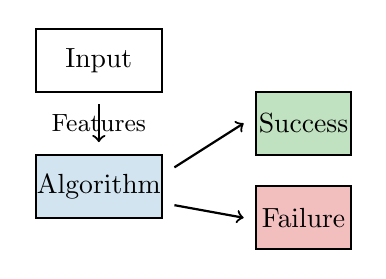
\begin{tikzpicture}[scale=0.8]
% Input box
\draw[thick] (0,3) rectangle (2,4);
\node at (1,3.5) {Input};
\node[below] at (1,2.8) {\small Features};

% Computer/Algorithm
\draw[thick,fill=mlblue!20] (0,1) rectangle (2,2);
\node at (1,1.5) {Algorithm};

% Output boxes
\draw[thick,fill=mlgreen!30] (3.5,2) rectangle (5,3);
\node at (4.25,2.5) {Success};
\draw[thick,fill=mlred!30] (3.5,0.5) rectangle (5,1.5);
\node at (4.25,1) {Failure};

% Arrows
\draw[thick,->] (1,2.8) -- (1,2.2);
\draw[thick,->] (2.2,1.8) -- (3.3,2.5);
\draw[thick,->] (2.2,1.2) -- (3.3,1);
\end{tikzpicture}
\end{center}

\textbf{How it works:}
The computer learns patterns from examples, then applies those patterns to new cases
\end{column}
\end{columns}
\end{frame}

% Slide 2: Simple scoring - Logistic Regression
\begin{frame}{Start Simple: The Scoring Method}
\Large\textbf{Like a Judge Giving Points}
\normalsize

\vspace{0.5em}

\begin{columns}[T]
\begin{column}{0.48\textwidth}
\textbf{How It Works:}
\begin{enumerate}
\item Give points for good features
\item Subtract points for bad features
\item Add up total score (0-100)
\item Decide: Above 50? Success!
\end{enumerate}

\vspace{0.5em}
\textbf{Example Scoring:}
\begin{itemize}
\item High novelty: +30 points
\item Large market: +25 points
\item Strong team: +20 points
\item Long timeline: -10 points
\item \textbf{Total: 65 points → Success!}
\end{itemize}
\end{column}
\begin{column}{0.48\textwidth}
\begin{center}
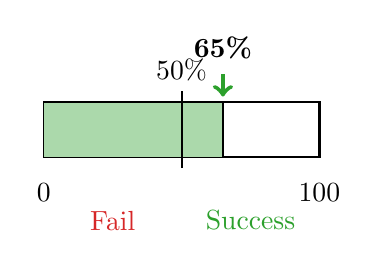
\begin{tikzpicture}[scale=0.7]
% Score bar
\draw[thick] (0,0) rectangle (5,1);
\draw[fill=mlgreen!40] (0,0) rectangle (3.25,1);

% Markers
\draw[thick] (2.5,-0.2) -- (2.5,1.2);
\node[above] at (2.5,1.2) {50\%};

% Score pointer
\draw[ultra thick,mlgreen,->] (3.25,1.5) -- (3.25,1.1);
\node[above] at (3.25,1.6) {\textbf{65\%}};

% Labels
\node[below] at (0,-0.3) {0};
\node[below] at (5,-0.3) {100};
\node[below] at (1.25,-0.8) {\textcolor{mlred}{Fail}};
\node[below] at (3.75,-0.8) {\textcolor{mlgreen}{Success}};
\end{tikzpicture}
\end{center}

\vspace{0.5em}
\textbf{Pros:}
\begin{itemize}
\item Very fast (instant results)
\item Easy to understand why
\item Good starting point
\end{itemize}

\textbf{Success Rate:} 76 out of 100 correct
\end{column}
\end{columns}
\end{frame}

% Slide 3: Decision Trees - 20 Questions
\begin{frame}{Playing 20 Questions: Decision Trees}
\Large\textbf{Computer Asks Yes/No Questions}
\normalsize

\vspace{0.5em}

\begin{columns}[T]
\begin{column}{0.55\textwidth}
\begin{center}
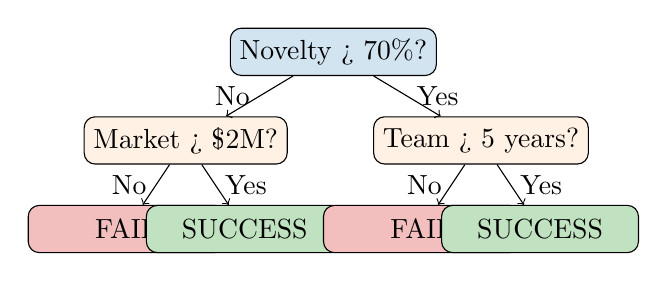
\begin{tikzpicture}[scale=0.75,
    box/.style={draw,rounded corners,minimum width=2.5cm,minimum height=0.6cm}]

% Root question
\node[box,fill=mlblue!20] (root) at (0,3) {Novelty > 70\%?};

% Second level
\node[box,fill=mlyellow!20] (left) at (-2.5,1.5) {Market > \$2M?};
\node[box,fill=mlyellow!20] (right) at (2.5,1.5) {Team > 5 years?};

% Outcomes
\node[box,fill=mlred!30] (ll) at (-3.5,0) {FAIL};
\node[box,fill=mlgreen!30] (lr) at (-1.5,0) {SUCCESS};
\node[box,fill=mlred!30] (rl) at (1.5,0) {FAIL};
\node[box,fill=mlgreen!30] (rr) at (3.5,0) {SUCCESS};

% Connections
\draw[->] (root) -- node[left] {No} (left);
\draw[->] (root) -- node[right] {Yes} (right);
\draw[->] (left) -- node[left] {No} (ll);
\draw[->] (left) -- node[right] {Yes} (lr);
\draw[->] (right) -- node[left] {No} (rl);
\draw[->] (right) -- node[right] {Yes} (rr);
\end{tikzpicture}
\end{center}
\end{column}
\begin{column}{0.43\textwidth}
\textbf{Like a Flowchart:}
\begin{itemize}
\item Start at the top
\item Answer each question
\item Follow the path
\item Reach a decision
\end{itemize}

\vspace{0.5em}
\textbf{Real Example:}
\begin{small}
\begin{enumerate}
\item Is it innovative? → Yes
\item Experienced team? → Yes
\item Result: \textcolor{mlgreen}{Likely Success!}
\end{enumerate}
\end{small}

\vspace{0.5em}
\textbf{Success Rate:} 79 out of 100 correct
\end{column}
\end{columns}
\end{frame}

% Slide 4: Random Forest - Wisdom of Crowds
\begin{frame}{Ask 100 Experts: Random Forest}
\Large\textbf{Many Trees = Better Decisions}
\normalsize

\vspace{0.5em}

\begin{columns}[T]
\begin{column}{0.48\textwidth}
\textbf{The Wisdom of Crowds:}
\begin{itemize}
\item Create 100 different decision trees
\item Each tree votes: Success or Fail
\item Take the majority vote
\item More reliable than one tree alone
\end{itemize}

\vspace{0.5em}
\textbf{Why It Works:}
\begin{itemize}
\item Different trees catch different patterns
\item Errors cancel out
\item Very hard to fool
\item Works on complex problems
\end{itemize}
\end{column}
\begin{column}{0.48\textwidth}
\begin{center}
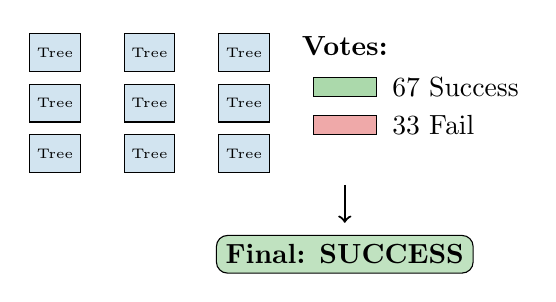
\begin{tikzpicture}[scale=0.8]
% Trees voting
\foreach \x in {0,1,2} {
    \foreach \y in {0,1,2} {
        \draw[fill=mlblue!20] (\x*1.5,\y*0.8) rectangle (\x*1.5+0.8,\y*0.8+0.6);
        \node at (\x*1.5+0.4,\y*0.8+0.3) {\tiny Tree};
    }
}

% Votes
\node at (5,2) {\textbf{Votes:}};
\draw[fill=mlgreen!40] (4.5,1.2) rectangle (5.5,1.5);
\node[right] at (5.6,1.35) {67 Success};
\draw[fill=mlred!40] (4.5,0.6) rectangle (5.5,0.9);
\node[right] at (5.6,0.75) {33 Fail};

% Arrow and result
\draw[thick,->] (5,-0.2) -- (5,-0.8);
\node[draw,fill=mlgreen!30,rounded corners] at (5,-1.3) {\textbf{Final: SUCCESS}};
\end{tikzpicture}
\end{center}

\vspace{0.5em}
\textbf{Success Rate:} 86 out of 100 correct
\end{column}
\end{columns}
\end{frame}

% Slide 5: SVM - Finding the best separator
\begin{frame}{Drawing the Best Line: Support Vectors}
\Large\textbf{Maximum Separation Strategy}
\normalsize

\vspace{0.5em}

\begin{columns}[T]
\begin{column}{0.48\textwidth}
\textbf{The Concept:}
\begin{itemize}
\item Find the widest "street" between groups
\item Like separating red and green marbles
\item Maximize the gap for safety
\item Works even with curved boundaries
\end{itemize}

\vspace{0.5em}
\textbf{Imagine:}
Drawing a line to separate two neighborhoods - you want the widest possible road between them

\vspace{0.5em}
\textbf{Success Rate:} 84 out of 100 correct
\end{column}
\begin{column}{0.48\textwidth}
\begin{center}
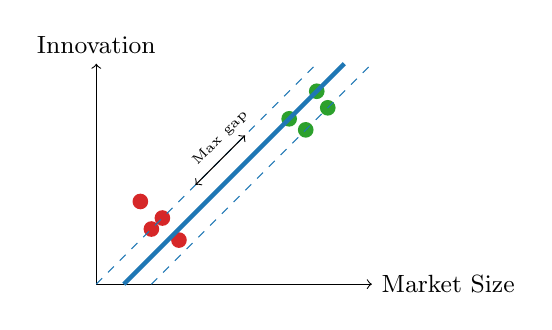
\begin{tikzpicture}[scale=0.7]
% Axes
\draw[->] (0,0) -- (5,0) node[right] {\small Market Size};
\draw[->] (0,0) -- (0,4) node[above] {\small Innovation};

% Success points
\foreach \x/\y in {3.5/3, 4/3.5, 3.8/2.8, 4.2/3.2} {
    \node[circle,fill=mlgreen,inner sep=2pt] at (\x,\y) {};
}

% Failure points
\foreach \x/\y in {1/1, 1.5/0.8, 0.8/1.5, 1.2/1.2} {
    \node[circle,fill=mlred,inner sep=2pt] at (\x,\y) {};
}

% Decision boundary
\draw[ultra thick,mlblue] (0.5,0) -- (4.5,4);

% Margin
\draw[dashed,mlblue] (0,0) -- (4,4);
\draw[dashed,mlblue] (1,0) -- (5,4);

% Annotation
\draw[<->] (1.8,1.8) -- (2.7,2.7);
\node[rotate=45] at (2.25,2.65) {\tiny Max gap};
\end{tikzpicture}
\end{center}

\textbf{Key Insight:}
The algorithm finds the safest boundary with maximum margin for error
\end{column}
\end{columns}
\end{frame}

% Slide 6: Neural Networks - Pattern recognition
\begin{frame}{Learning Like a Brain: Neural Networks}
\Large\textbf{Finding Complex Patterns}
\normalsize

\vspace{0.5em}

\begin{columns}[T]
\begin{column}{0.48\textwidth}
\textbf{Inspired by the Brain:}
\begin{itemize}
\item Multiple layers of "neurons"
\item Each layer learns different patterns
\item Combines simple patterns into complex ones
\item Can learn almost any relationship
\end{itemize}

\vspace{0.5em}
\textbf{Think of it as:}
\begin{itemize}
\item Layer 1: Sees basic features
\item Layer 2: Combines basics
\item Layer 3: Makes final decision
\end{itemize}
\end{column}
\begin{column}{0.48\textwidth}
\begin{center}
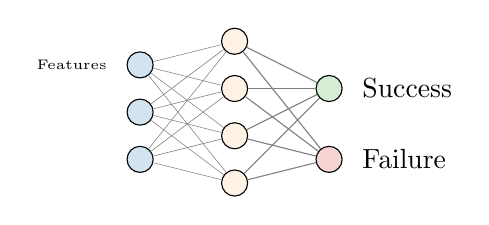
\begin{tikzpicture}[scale=0.6]
% Input layer
\node[circle,draw,fill=mlblue!20] (i1) at (0,1) {};
\node[circle,draw,fill=mlblue!20] (i2) at (0,2) {};
\node[circle,draw,fill=mlblue!20] (i3) at (0,3) {};
\node[left] at (-0.5,3) {\tiny Features};

% Hidden layer
\node[circle,draw,fill=mlyellow!20] (h1) at (2,0.5) {};
\node[circle,draw,fill=mlyellow!20] (h2) at (2,1.5) {};
\node[circle,draw,fill=mlyellow!20] (h3) at (2,2.5) {};
\node[circle,draw,fill=mlyellow!20] (h4) at (2,3.5) {};

% Output layer
\node[circle,draw,fill=mlgreen!20] (o1) at (4,2.5) {};
\node[circle,draw,fill=mlred!20] (o2) at (4,1) {};

% Connections (simplified)
\foreach \i in {1,2,3} {
    \foreach \j in {1,2,3,4} {
        \draw[gray,very thin] (i\i) -- (h\j);
    }
}
\foreach \j in {1,2,3,4} {
    \draw[gray] (h\j) -- (o1);
    \draw[gray] (h\j) -- (o2);
}

% Labels
\node[right] at (4.5,2.5) {Success};
\node[right] at (4.5,1) {Failure};
\end{tikzpicture}
\end{center}

\vspace{0.5em}
\textbf{Pros:} Very accurate on complex data\\
\textbf{Cons:} Hard to explain why it decided\\
\textbf{Success Rate:} 88 out of 100 correct
\end{column}
\end{columns}
\end{frame}

% Slide 7: Gradient Boosting - Learning from mistakes
\begin{frame}{Learning from Mistakes: Gradient Boosting}
\Large\textbf{Getting Better Step by Step}
\normalsize

\vspace{0.5em}

\begin{columns}[T]
\begin{column}{0.48\textwidth}
\textbf{The Learning Process:}
\begin{enumerate}
\item Make initial predictions
\item Find where you were wrong
\item Focus on fixing those mistakes
\item Repeat until very accurate
\end{enumerate}

\vspace{0.5em}
\textbf{Like Studying for a Test:}
\begin{itemize}
\item Take practice exam
\item Study what you got wrong
\item Take another practice exam
\item Keep improving weak areas
\end{itemize}
\end{column}
\begin{column}{0.48\textwidth}
\begin{center}
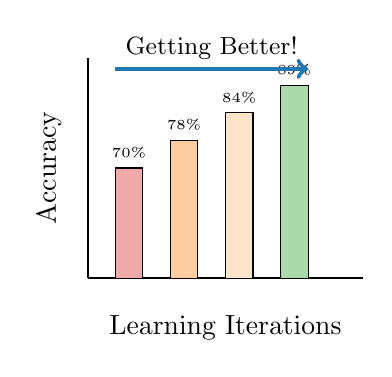
\begin{tikzpicture}[scale=0.7]
% Iteration bars showing improvement
\draw[thick] (0,0) -- (0,4);
\draw[thick] (0,0) -- (5,0);

% Accuracy bars
\draw[fill=mlred!40] (0.5,0) rectangle (1,2);
\node[above] at (0.75,2) {\tiny 70\%};

\draw[fill=mlorange!40] (1.5,0) rectangle (2,2.5);
\node[above] at (1.75,2.5) {\tiny 78\%};

\draw[fill=mlyellow!40] (2.5,0) rectangle (3,3);
\node[above] at (2.75,3) {\tiny 84\%};

\draw[fill=mlgreen!40] (3.5,0) rectangle (4,3.5);
\node[above] at (3.75,3.5) {\tiny 89\%};

% Labels
\node[below] at (2.5,-0.5) {Learning Iterations};
\node[rotate=90] at (-0.7,2) {Accuracy};

% Arrow showing improvement
\draw[ultra thick,->,mlblue] (0.5,3.8) -- (4,3.8);
\node[above] at (2.25,3.8) {\small Getting Better!};
\end{tikzpicture}
\end{center}

\textbf{Success Rate:} 89 out of 100 correct\\
\textbf{Best performer} in most cases!
\end{column}
\end{columns}
\end{frame}

% Slide 8: Algorithm Showdown - Simplified comparison
\begin{frame}{Algorithm Showdown}
\Large\textbf{Which Method Should You Choose?}
\normalsize

\vspace{0.5em}

\begin{center}
% Simple visual comparison
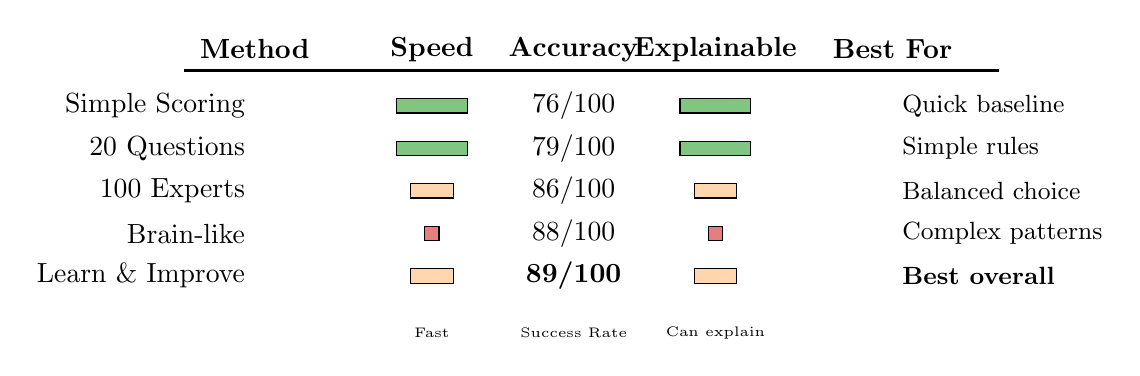
\begin{tikzpicture}[scale=0.9]
% Title row
\node at (0,4) {\textbf{Method}};
\node at (2.5,4) {\textbf{Speed}};
\node at (4.5,4) {\textbf{Accuracy}};
\node at (6.5,4) {\textbf{Explainable}};
\node at (9,4) {\textbf{Best For}};

\draw[thick] (-1,3.7) -- (10.5,3.7);

% Scoring Method
\node[left] at (0,3.2) {Simple Scoring};
\draw[fill=mlgreen!60] (2,3.1) rectangle (3,3.3); % Fast
\node at (4.5,3.2) {76/100};
\draw[fill=mlgreen!60] (6,3.1) rectangle (7,3.3); % Explainable
\node[right] at (9,3.2) {\small Quick baseline};

% Decision Tree
\node[left] at (0,2.6) {20 Questions};
\draw[fill=mlgreen!60] (2,2.5) rectangle (3,2.7); % Fast
\node at (4.5,2.6) {79/100};
\draw[fill=mlgreen!60] (6,2.5) rectangle (7,2.7); % Explainable
\node[right] at (9,2.6) {\small Simple rules};

% Random Forest
\node[left] at (0,2) {100 Experts};
\draw[fill=mlyellow!60] (2.2,1.9) rectangle (2.8,2.1); % Medium
\node at (4.5,2) {86/100};
\draw[fill=mlyellow!60] (6.2,1.9) rectangle (6.8,2.1); % Somewhat
\node[right] at (9,2) {\small Balanced choice};

% Neural Network
\node[left] at (0,1.4) {Brain-like};
\draw[fill=mlred!60] (2.4,1.3) rectangle (2.6,1.5); % Slow
\node at (4.5,1.4) {88/100};
\draw[fill=mlred!60] (6.4,1.3) rectangle (6.6,1.5); % Not explainable
\node[right] at (9,1.4) {\small Complex patterns};

% Gradient Boosting
\node[left] at (0,0.8) {Learn \& Improve};
\draw[fill=mlyellow!60] (2.2,0.7) rectangle (2.8,0.9); % Medium
\node at (4.5,0.8) {\textbf{89/100}};
\draw[fill=mlyellow!60] (6.2,0.7) rectangle (6.8,0.9); % Somewhat
\node[right] at (9,0.8) {\small \textbf{Best overall}};

% Legend
\node at (2.5,0) {\tiny Fast};
\node at (4.5,0) {\tiny Success Rate};
\node at (6.5,0) {\tiny Can explain};
\end{tikzpicture}
\end{center}

\vspace{0.5em}

\begin{center}
\begin{tcolorbox}[colback=mlblue!10,colframe=mlblue,width=0.8\textwidth]
\textbf{Recommendation:} Start simple (Scoring), then try Random Forest or Gradient Boosting for better accuracy
\end{tcolorbox}
\end{center}
\end{frame}

% Slide 9: Metrics - What does success mean?
\begin{frame}{Measuring Success}
\Large\textbf{It's Not Just About Being Right}
\normalsize

\vspace{0.5em}

\begin{columns}[T]
\begin{column}{0.48\textwidth}
\textbf{Different Ways to Measure:}
\begin{itemize}
\item \textbf{Accuracy:} How many correct overall?
\item \textbf{Precision:} When you say "success", how often are you right?
\item \textbf{Recall:} Of all successes, how many did you find?
\end{itemize}

\vspace{0.5em}
\textbf{Real Example:}
\begin{itemize}
\item 100 startups evaluated
\item 10 actual successes
\item Algorithm found 8 of them
\item But also wrongly labeled 2 failures as success
\end{itemize}
\end{column}
\begin{column}{0.48\textwidth}
\begin{center}
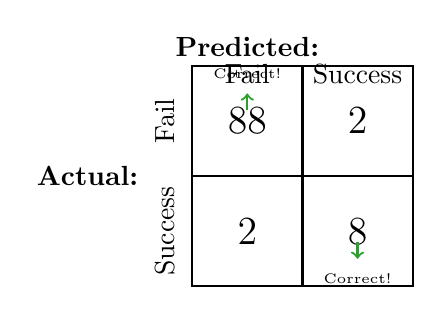
\begin{tikzpicture}[scale=0.7]
% Grid for confusion matrix
\draw[thick] (0,0) rectangle (4,4);
\draw[thick] (2,0) -- (2,4);
\draw[thick] (0,2) -- (4,2);

% Labels
\node[above] at (1,4) {\textbf{Predicted:}};
\node[above] at (1,3.5) {Fail};
\node[above] at (3,3.5) {Success};
\node[rotate=90] at (-0.5,3) {Fail};
\node[rotate=90] at (-0.5,1) {Success};
\node[left] at (-0.8,2) {\textbf{Actual:}};

% Numbers
\node at (1,3) {\Large 88};
\node at (3,3) {\Large 2};
\node at (1,1) {\Large 2};
\node at (3,1) {\Large 8};

% Annotations
\draw[->,thick,mlgreen] (1,3.2) -- (1,3.5);
\node[above] at (1,3.6) {\tiny Correct!};
\draw[->,thick,mlgreen] (3,0.8) -- (3,0.5);
\node[below] at (3,0.4) {\tiny Correct!};
\end{tikzpicture}
\end{center}

\textbf{Results:}
\begin{itemize}
\item Accuracy: 96\% (96/100 correct)
\item Precision: 80\% (8/10 predictions correct)
\item Recall: 80\% (8/10 successes found)
\end{itemize}
\end{column}
\end{columns}
\end{frame}

% Slide 10: ROC Curves - Simplified
\begin{frame}{Finding the Sweet Spot}
\Large\textbf{Balancing Different Types of Errors}
\normalsize

\vspace{0.5em}

\begin{columns}[T]
\begin{column}{0.48\textwidth}
\textbf{The Trade-off:}
\begin{itemize}
\item Be strict: Miss opportunities
\item Be lenient: Waste resources
\item Need to find balance
\end{itemize}

\vspace{0.5em}
\textbf{ROC Curve Shows:}
\begin{itemize}
\item How well algorithm separates groups
\item Where to set the threshold
\item Closer to top-left = better
\end{itemize}

\vspace{0.5em}
\textbf{Think of it as:}
Setting the bar for a high jump - too high and everyone fails, too low and everyone passes
\end{column}
\begin{column}{0.48\textwidth}
\begin{center}
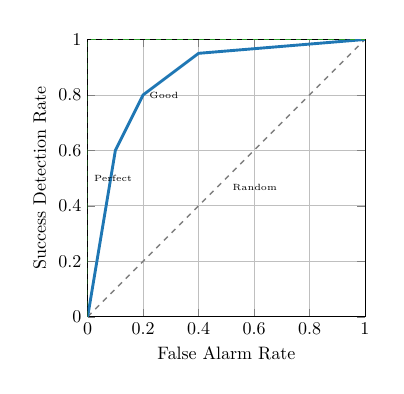
\begin{tikzpicture}[scale=0.65]
\begin{axis}[
    xlabel={False Alarm Rate},
    ylabel={Success Detection Rate},
    xmin=0, xmax=1,
    ymin=0, ymax=1,
    grid=major,
    width=7cm,
    height=7cm
]
% Random guess
\addplot[dashed,mlgray,thick] coordinates {(0,0) (1,1)};
% Good classifier
\addplot[mlblue,ultra thick] coordinates {
    (0,0) (0.05,0.3) (0.1,0.6) (0.2,0.8) (0.4,0.95) (1,1)
};
% Perfect classifier
\addplot[mlgreen,thick,dashed] coordinates {(0,0) (0,1) (1,1)};

% Annotations
\node at (axis cs:0.5,0.5) [below right] {\tiny Random};
\node at (axis cs:0.2,0.8) [right] {\tiny Good};
\node at (axis cs:0,0.5) [right] {\tiny Perfect};
\end{axis}
\end{tikzpicture}
\end{center}

The closer to the top-left corner, the better your algorithm!
\end{column}
\end{columns}
\end{frame}

% Slide 11: Imbalanced data
\begin{frame}{When Success is Rare}
\Large\textbf{The 5\% Challenge}
\normalsize

\vspace{0.5em}

\begin{columns}[T]
\begin{column}{0.48\textwidth}
\textbf{The Problem:}
\begin{itemize}
\item Only 5\% of startups succeed
\item Algorithm could just say "all fail"
\item Would be 95\% accurate!
\item But completely useless
\end{itemize}

\vspace{0.5em}
\textbf{Solutions:}
\begin{enumerate}
\item Give more weight to rare successes
\item Generate synthetic success examples
\item Use different metrics (not just accuracy)
\item Adjust the decision threshold
\end{enumerate}
\end{column}
\begin{column}{0.48\textwidth}
\begin{center}
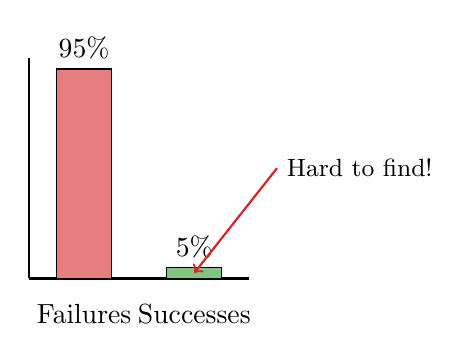
\begin{tikzpicture}[scale=0.7]
% Bar chart showing imbalance
\draw[thick] (0,0) -- (4,0);
\draw[thick] (0,0) -- (0,4);

% Bars
\draw[fill=mlred!60] (0.5,0) rectangle (1.5,3.8);
\node[above] at (1,3.8) {95\%};
\node[below] at (1,-0.3) {Failures};

\draw[fill=mlgreen!60] (2.5,0) rectangle (3.5,0.2);
\node[above] at (3,0.2) {5\%};
\node[below] at (3,-0.3) {Successes};

% Problem annotation
\draw[->,thick,mlred] (4.5,2) -- (3,0.1);
\node[right] at (4.5,2) {\small Hard to find!};
\end{tikzpicture}
\end{center}

\vspace{0.5em}
\textbf{Key Insight:}
With rare events, we need special techniques to ensure the algorithm learns to recognize them
\end{column}
\end{columns}
\end{frame}

% Slide 12: Transition to implementation
\begin{frame}{Ready to Build?}
\Large\textbf{From Understanding to Doing}
\normalsize

\vspace{1em}

\begin{center}
Now you understand how algorithms classify:
\begin{itemize}
\item Simple scoring to complex patterns
\item Different methods for different needs
\item How to measure success properly
\item Dealing with rare events
\end{itemize}

\vspace{1em}
\Huge\textbf{Next: Making It Work!}

\vspace{1em}
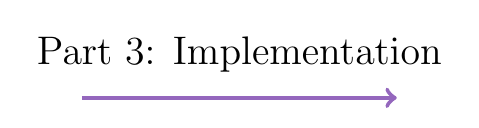
\begin{tikzpicture}
\draw[ultra thick,->,mlpurple] (0,0) -- (4,0);
\node[above] at (2,0.2) {\Large Part 3: Implementation};
\end{tikzpicture}

\vspace{1em}
\Large\textit{``Time to build your own classifier''}
\end{center}
\end{frame}
\input{part3_implementation_v3_beginner}
\input{part4_design_v2}

% Include appendix
% Appendix: Mathematical Foundations (3 slides)
\section*{Appendix: Mathematical Foundations}

% Slide A1: Logistic Regression Mathematics
\begin{frame}{Appendix: Logistic Regression Mathematics}
\Large\textbf{Gradient Descent Optimization}
\normalsize

\vspace{0.5em}

\textbf{Log-Likelihood Function:}
$$\ell(\beta) = \sum_{i=1}^n \left[ y_i \log(p_i) + (1-y_i) \log(1-p_i) \right]$$

where $p_i = \frac{1}{1 + e^{-\beta^T x_i}}$

\vspace{0.5em}
\textbf{Gradient:}
$$\frac{\partial \ell}{\partial \beta_j} = \sum_{i=1}^n (y_i - p_i) x_{ij}$$

\vspace{0.5em}
\textbf{Update Rule:}
$$\beta^{(t+1)} = \beta^{(t)} + \alpha \sum_{i=1}^n (y_i - p_i^{(t)}) x_i$$

\vspace{0.5em}
\textbf{Convergence:} When $||\nabla \ell|| < \epsilon$ or maximum iterations reached

\vspace{0.5em}
\textbf{Regularization:} Add penalty term $-\lambda ||\beta||^2$ to prevent overfitting
\end{frame}

% Slide A2: Information Theory for Trees
\begin{frame}{Appendix: Information Theory for Decision Trees}
\Large\textbf{Entropy and Information Gain}
\normalsize

\vspace{0.5em}

\textbf{Entropy (Impurity Measure):}
$$H(S) = -\sum_{c \in C} p_c \log_2(p_c)$$

where $p_c$ is the proportion of samples in class $c$

\vspace{0.5em}
\textbf{Information Gain:}
$$IG(S, A) = H(S) - \sum_{v \in Values(A)} \frac{|S_v|}{|S|} H(S_v)$$

\vspace{0.5em}
\textbf{Gini Impurity (Alternative):}
$$Gini(S) = 1 - \sum_{c \in C} p_c^2$$

\vspace{0.5em}
\textbf{Example Calculation:}
\begin{columns}[T]
\begin{column}{0.48\textwidth}
Parent node: 60 success, 40 fail \\
$H(parent) = -0.6 \log_2(0.6) - 0.4 \log_2(0.4)$ \\
$H(parent) = 0.971$
\end{column}
\begin{column}{0.48\textwidth}
After split: \\
Left: 50 success, 10 fail \\
Right: 10 success, 30 fail \\
$IG = 0.971 - 0.811 = 0.160$
\end{column}
\end{columns}
\end{frame}

% Slide A3: SVM and Kernel Mathematics
\begin{frame}{Appendix: SVM and the Kernel Trick}
\Large\textbf{Maximum Margin Optimization}
\normalsize

\vspace{0.5em}

\textbf{Primal Optimization Problem:}
$$\min_{w,b} \frac{1}{2}||w||^2 \quad \text{subject to} \quad y_i(w^T x_i + b) \geq 1$$

\vspace{0.5em}
\textbf{Dual Form (Using Lagrange Multipliers):}
$$\max_{\alpha} \sum_{i=1}^n \alpha_i - \frac{1}{2}\sum_{i,j} \alpha_i \alpha_j y_i y_j x_i^T x_j$$

\vspace{0.5em}
\textbf{Kernel Trick:}
Replace $x_i^T x_j$ with kernel function $K(x_i, x_j)$

\vspace{0.5em}
\textbf{Common Kernels:}
\begin{itemize}
\item Linear: $K(x_i, x_j) = x_i^T x_j$
\item Polynomial: $K(x_i, x_j) = (x_i^T x_j + r)^d$
\item RBF (Gaussian): $K(x_i, x_j) = \exp(-\gamma ||x_i - x_j||^2)$
\item Sigmoid: $K(x_i, x_j) = \tanh(\kappa x_i^T x_j + c)$
\end{itemize}

\vspace{0.5em}
\textbf{Decision Function:}
$$f(x) = \text{sign}\left(\sum_{i \in SV} \alpha_i y_i K(x_i, x) + b\right)$$
\end{frame}

% Closing slide
\begin{frame}[plain]
\begin{center}
\Huge\textbf{Thank You!}

\vspace{1em}
\Large
Questions?

\vspace{2em}
\normalsize
Remember: Everyone starts as a beginner!

\vspace{1em}
innovation-ml-course@university.edu
\end{center}
\end{frame}

\end{document}